\section{Descripción de la solución}\label{sec:solution}


\subsection{Alternativa seleccionada}
\par Por todo lo visto a lo largo de la sección \ref{sec:alt}, se ha considerado que la mejor solución posible para el desarrollo de \textit{IRMASpace} es el uso de Liferay, ya que su uso está muy extendido en el mercado, su coste es aceptable y el tiempo de desarrollo del proyecto está dentro de los límites de viabilidad.

\subsection{Características de Liferay}
\par Una vez seleccionada la alternativa como mejor solución, es necesario especificar más aún sus funcionalidades, arquitectura , tecnologías y características en general.

\subsubsection{Arquitectura}
\par Para explicar de manera ordenada la arquitectura de Liferay la dividiremos en los usuarios y sus roles, las organizaciones, el Web Site, los equipos y los permisos.
\begin{itemize}
    \item Usuarios: personas físicas que usan el sistema. Estos pueden acceder a los portales. Así mismo, los usuarios pertenecen a organizaciones.
    \item Organizaciones: pueden establecerse como una jerarquía.
    \item Web Site: conjunto de usuarios sin jerarquía.
    \item Equipos: dentro de una Web Site u Organización, los usuarios pertenecientes a las mismas pueden organizarse mediante equipos jerarquizados o no.
    \item Roles: conjunto de permisos de los usuarios sobre los objetos. Por defecto, existen tres tipos de roles: roles de portal, roles de organización y roles de sitio web. En la imagen \ref{img:roles} puede verse esta definición con más claridad.
    \begin{figure}[H]
    \begin{center}
    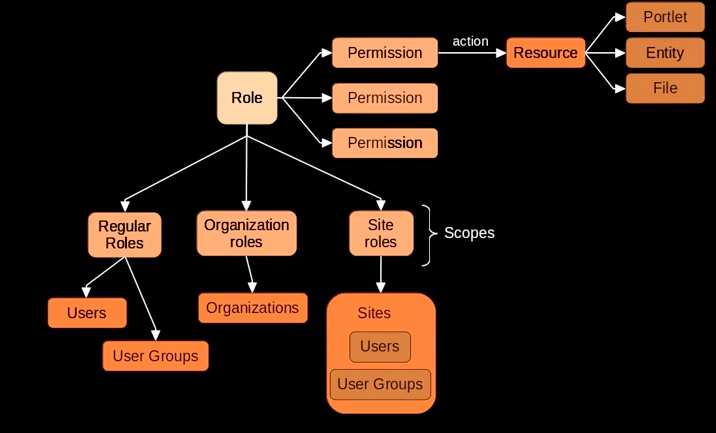
\includegraphics[width=0.7\textwidth]{./img/liferay_roles.png}
    \end{center}
    \caption{Roles en Liferay}
    \label{img:roles}
    \end{figure}

    \item Permisos: diferentes acciones que un usuario puede realizar sobre un recurso.
\end{itemize}
\par Se puede ver una visión global de la arquitectura de Liferay en la imagen \ref{img:arch}.
\begin{figure}[H]
\begin{center}
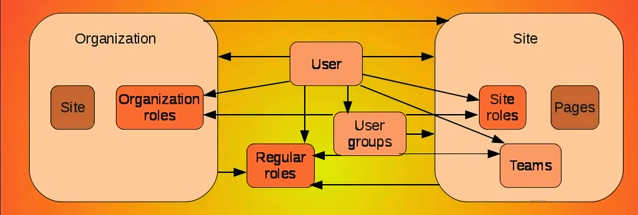
\includegraphics[width=0.7\textwidth]{./img/liferay_arch.png}
\end{center}
\caption{Arquitectura de Liferay}
\label{img:arch}
\end{figure}

\subsubsection{Tecnologías}
\par Liferay permite realizar diseños responsivos y adaptables a cualquier tipo de dispositivo mediante la compatibilidad con HTML5, CSS3, Bootstrap y jQuery. Ello permite realizar Portales Web accesibles.
\par Así mismo, dispone de un Entorno Integrado de Desarrollo bajo arquitectura Java, lo que lo hace compatible con las tecnologías de Orache, MySQL, Spring y JSF entre otros.
\par La arquitectura de Liferay es orientada a servicios, por lo que dispone de una plataforma SOA, haciendo de Liferay una herramienta muy adecuada para desarrollo de aplicaciones coorporativas.
\subsubsection{Funcionalidades y componentes}
\par En cuanto a las funcionalidad y componentes para el desarrollo de un Portal se refiere, se pueden encontrar los siguientes aspectos a destacar:
\begin{itemize}
    \item Framework de integración de aplicaciones.
    \item Soporte de Single Sign One (SSO) que facilita la autenticación una única vez.
    \item Soporte para campos personalizados desde la interfaz gráfica sin necesidad de modificar la base de datos.
    \item Publicación de contenidos basada en roles, tal y como se vio en la Arquitectura de Liferay.
    \item Interfaz gráfica de gran agilidad y flexibilidad, apoyándose en la administración mediante \textit{Drag & Drop}.
    \item Framework de WorkFlow dirigido por el usuario que permite definir procesos de publicación y aprobación.
    \item Sincronización de archivos mediante Liferay Sync
    \item Soporte Multi-idioma
    \item Mecanismos de contribución sociales integrados en OpenSocial.
\end{itemize}

\par Todo ello ofrece grandes ventajas para los usuarios de Liferay. Algunas de estas ventajas pueden ser:
\begin{itemize}
    \item Repositorio de documentos y archivos multimedia único.
    \item Publicador de contenidos que puede ser añadido a cualquier página web.
    \item Editores avanzados de texto con corrección ortográfica y definición de estilos.
    \item Estructuras y plantillas predefinidas y reutilizables.
    \item Integración con Microsoft Office.
    \item Publicación inmediata y planificada.
\end{itemize}
